\subsection{Smoothing}
\begin{figure}[H]
	\centering
	\begin{subfigure}{0.45\textwidth}
	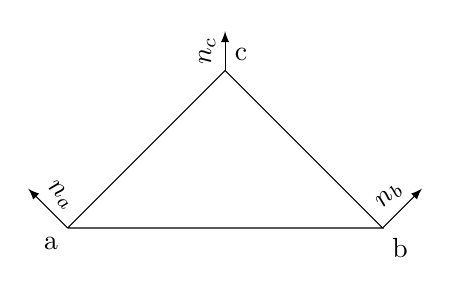
\begin{tikzpicture}[scale=2]
	\draw (-1,0) node[anchor=north east] {a}--(1,0) node[anchor=north west] {b}--(0,1) node[anchor=south west] {c}--(-1,0);
	\draw[-latex] (-1,0)--(-1.25,.25) node[above, pos=.5, sloped] {$n_a$};
	\draw[-latex] (1,0)--(1.25,.25) node[above, pos=.5, sloped] {$n_b$};
	\draw[-latex] (0,1)--(0,1.25) node[above, pos=.5, sloped] {$n_c$};
	\end{tikzpicture}
\end{subfigure}
\begin{subfigure}{0.45\textwidth}
	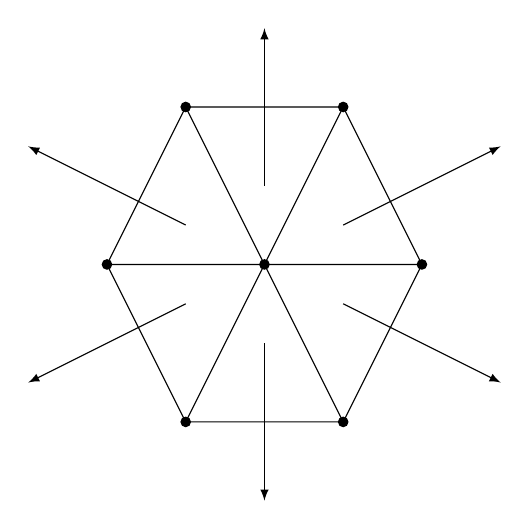
\begin{tikzpicture}[scale=2]
	\draw (-1,0)--(-.5,1)--(.5,1)--(1,0)--(.5,-1)--(-.5,-1)--(-1,0)
	(-1,0)--(0,0)
	(-.5,1)--(0,0)
	(.5,1)--(0,0)
	(1,0)--(0,0)
	(.5,-1)--(0,0)
	(-.5,-1)--(0,0);
	\filldraw
	(-1,0)circle (0.03)
	(-.5,1)circle (0.03)
	(.5,1)circle (0.03)
	(1,0)circle (0.03)
	(.5,-1)circle (0.03)
	(-.5,-1)circle (0.03)
	(0,0)circle (0.03);
	\draw[-latex] (0,.5)--(0,1.5);
	\draw[-latex] (-.5,.25)--(-1.5,.75);
	\draw[-latex] (-.5,-.25)--(-1.5,-.75);
	\draw[-latex] (0,-.5)--(0,-1.5);
	\draw[-latex] (.5,.25)--(1.5,.75);
	\draw[-latex] (.5,-.25)--(1.5,-.75);
%	\draw[-latex] (-1,0)--(-1.25,.25) node[above, pos=.5, sloped] {$n_a$};
%	\draw[-latex] (1,0)--(1.25,.25) node[above, pos=.5, sloped] {$n_b$};
%	\draw[-latex] (0,1)--(0,1.25) node[above, pos=.5, sloped] {$n_c$};
	\end{tikzpicture}
	
	\end{subfigure}
\end{figure}
\pagebreak
\subsubsection{Lambert}
\[ \text{I}_D = \text{I}_L \cdot \left( n^T \cdot \ell \right) \]
\begin{figure}[H]
	\centering
	\begin{tikzpicture}
	\draw (-1,0)--(1,0);
	\draw[-latex] (0,0) node (b){}--(0,1) node(c){};
	\draw[-latex] (0,0)--(0.707,0.707)node(a){};
	\draw pic[draw, "$\varphi$" , angle eccentricity=1.2, angle radius=15] {angle=a--b--c};
	\draw[dashed] (0.707,0.707)--(2*0.707,2*0.707)node[scale=0.05,solid, draw,star,star points=12,star point ratio=28]{};
	\end{tikzpicture}
\end{figure}